\chapter{Projectactiviteiten}

\section{Mijlpalen en Planning}
\subsection{Mijlpalen}
Hieronder vind u de planning voor het gehele project. De genoemde data zijn de deadlines voor oplevering en reflecteren niet de werkelijke inleverdatum.
\begin{table}[]
\centering
\begin{tabular}{ l c r }
  Teamcontract & 11-11-2015 (Week 1) \\
  Github Repo (met bijbehorende mappen) & 11-11-2015 (Week 1) \\
  Interview Opdrachtgever & 30-11-2015 (Week 3) \\
  Plan van Aanpak & 02-12-2015 (Week 4) \\
  Requirements Document (MoSCoW) & 01-12-2015 (Week 4) \\
  Requirements Architechture &  09-12-2015 (Week 5) \\
  Solution Architechture & 16-12-2015 (Week 6) \\
  Technisch Verslag	& (Week 7 / Projectweek 1) \\
  Eindproduct (software + hardware)	& 22-01-2016 \\
\end{tabular}
\end{table}

\subsection{Planning}
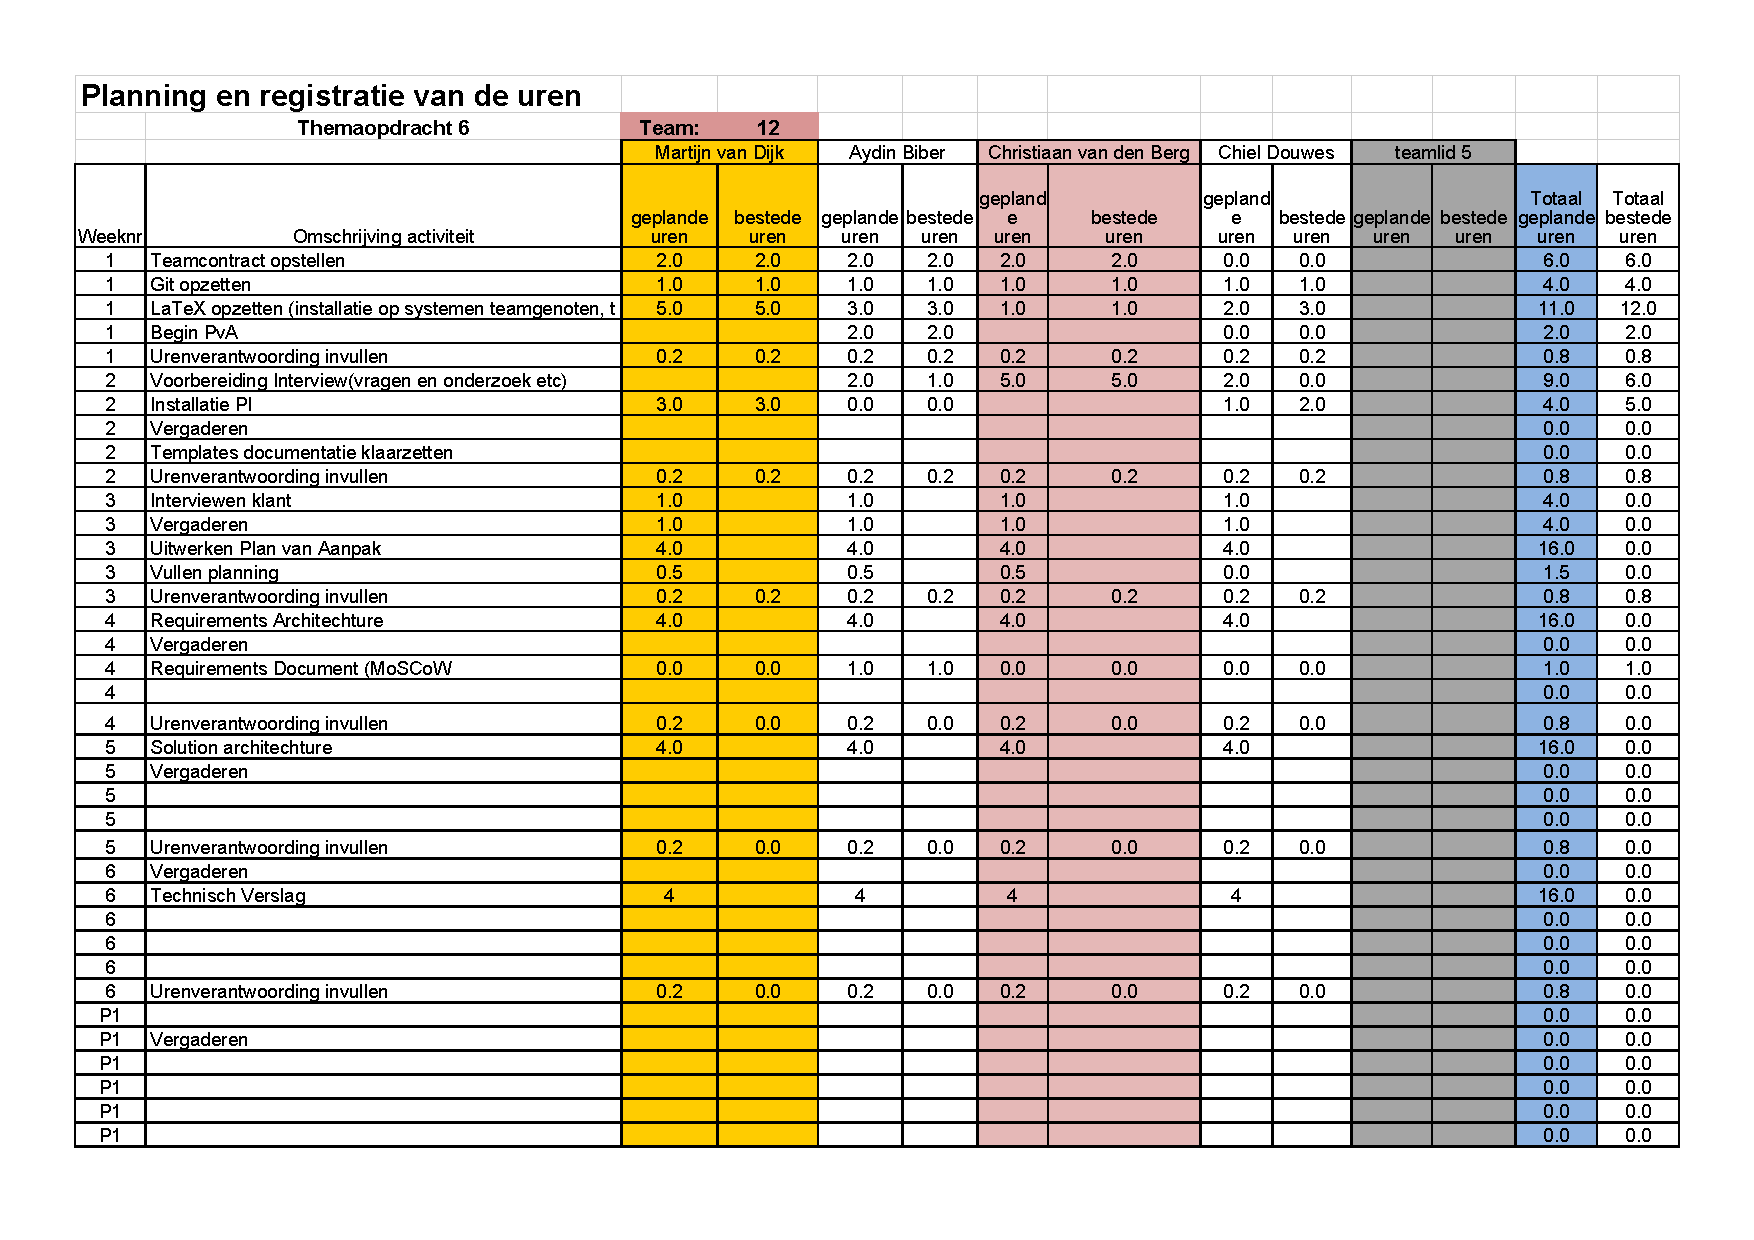
\includepdf[pages=-, landscape=true]{Chapters/urenplanning.pdf}